\documentclass[11pt]{article}

\usepackage[margin=2cm]{geometry}

\usepackage{graphicx}

\usepackage{booktabs}

\usepackage{hyperref}

\usepackage[T1]{fontenc}

\usepackage[utf8]{inputenc}

\title{Foco textil estricto Santa Ana Xalmimilulco 2026}

\author{Proyecto Atoyac - salida reproducible}

\date{\today}

\begin{document}

\maketitle

\section{Proposito}

Este reporte corrige el universo foco amplio para Santa Ana Xalmimilulco. El producto nuevo se llama \texttt{foco\_textil\_estricto\_santa\_ana\_2026} y se limita a establecimientos con senales de tratamiento, lavado, tintoreria, acabado, mezclilla, jeans, deshebrado o produccion material textil. No es una prueba de descarga ni contaminacion.

\section{Criterio estricto}

Se partio de \texttt{data/processed/denue2026\_universo\_textil\_clasificado.gpkg} y se filtro exclusivamente la localidad Santa Ana Xalmimilulco. Se excluyeron planchado, confeccion o alta costura, ropa terminada generica, talleres sin senal especifica, lavados no textiles, insumos para lavanderia, bodegas, servicios de agua y actividades no textiles. La senal de mezclilla/deshebrado se exigio en el nombre del establecimiento o en la etapa productiva ya clasificada.

\section{Resultados}

El foco estricto contiene 67 registros. Del foco amplio de Santa Ana salen 273 registros.

\subsection{Categorias incluidas}

\begin{tabular}{ll}
\toprule
categoria\_foco\_estricto & registros \\
\midrule
mezclilla\_jeans\_deshebrado & 44 \\
tratamiento\_lavado\_acabado\_textil & 23 \\
\bottomrule
\end{tabular}

\subsection{Membresias}

\begin{tabular}{ll}
\toprule
conjunto & registros \\
\midrule
foco\_textil\_estricto\_santa\_ana\_2026 & 67 \\
en\_universo\_prioritario\_2026\_santa\_ana & 37 \\
en\_universo\_prioritario\_actual\_santa\_ana & 34 \\
en\_mh\_filtrado & 11 \\
\bottomrule
\end{tabular}

\subsection{Comparacion con MH filtrado}

\begin{tabular}{ll}
\toprule
comparacion\_estricto\_mh & registros \\
\midrule
estricto\_y\_mh & 11 \\
mh\_sin\_id & 6 \\
solo\_estricto & 56 \\
solo\_mh & 32 \\
\bottomrule
\end{tabular}

\subsection{Registros excluidos del foco amplio}

\begin{tabular}{ll}
\toprule
motivo\_exclusion\_foco\_estricto & registros \\
\midrule
confeccion\_maquila\_generica & 233 \\
planchado\_o\_costura\_especializada & 17 \\
pendiente\_sin\_senal\_estricta & 10 \\
bordado\_o\_textil\_ligero & 8 \\
servicio\_insumo\_bodega\_no\_proceso & 5 \\
\bottomrule
\end{tabular}

\section{Mapas}

\begin{figure}[h!]\centering

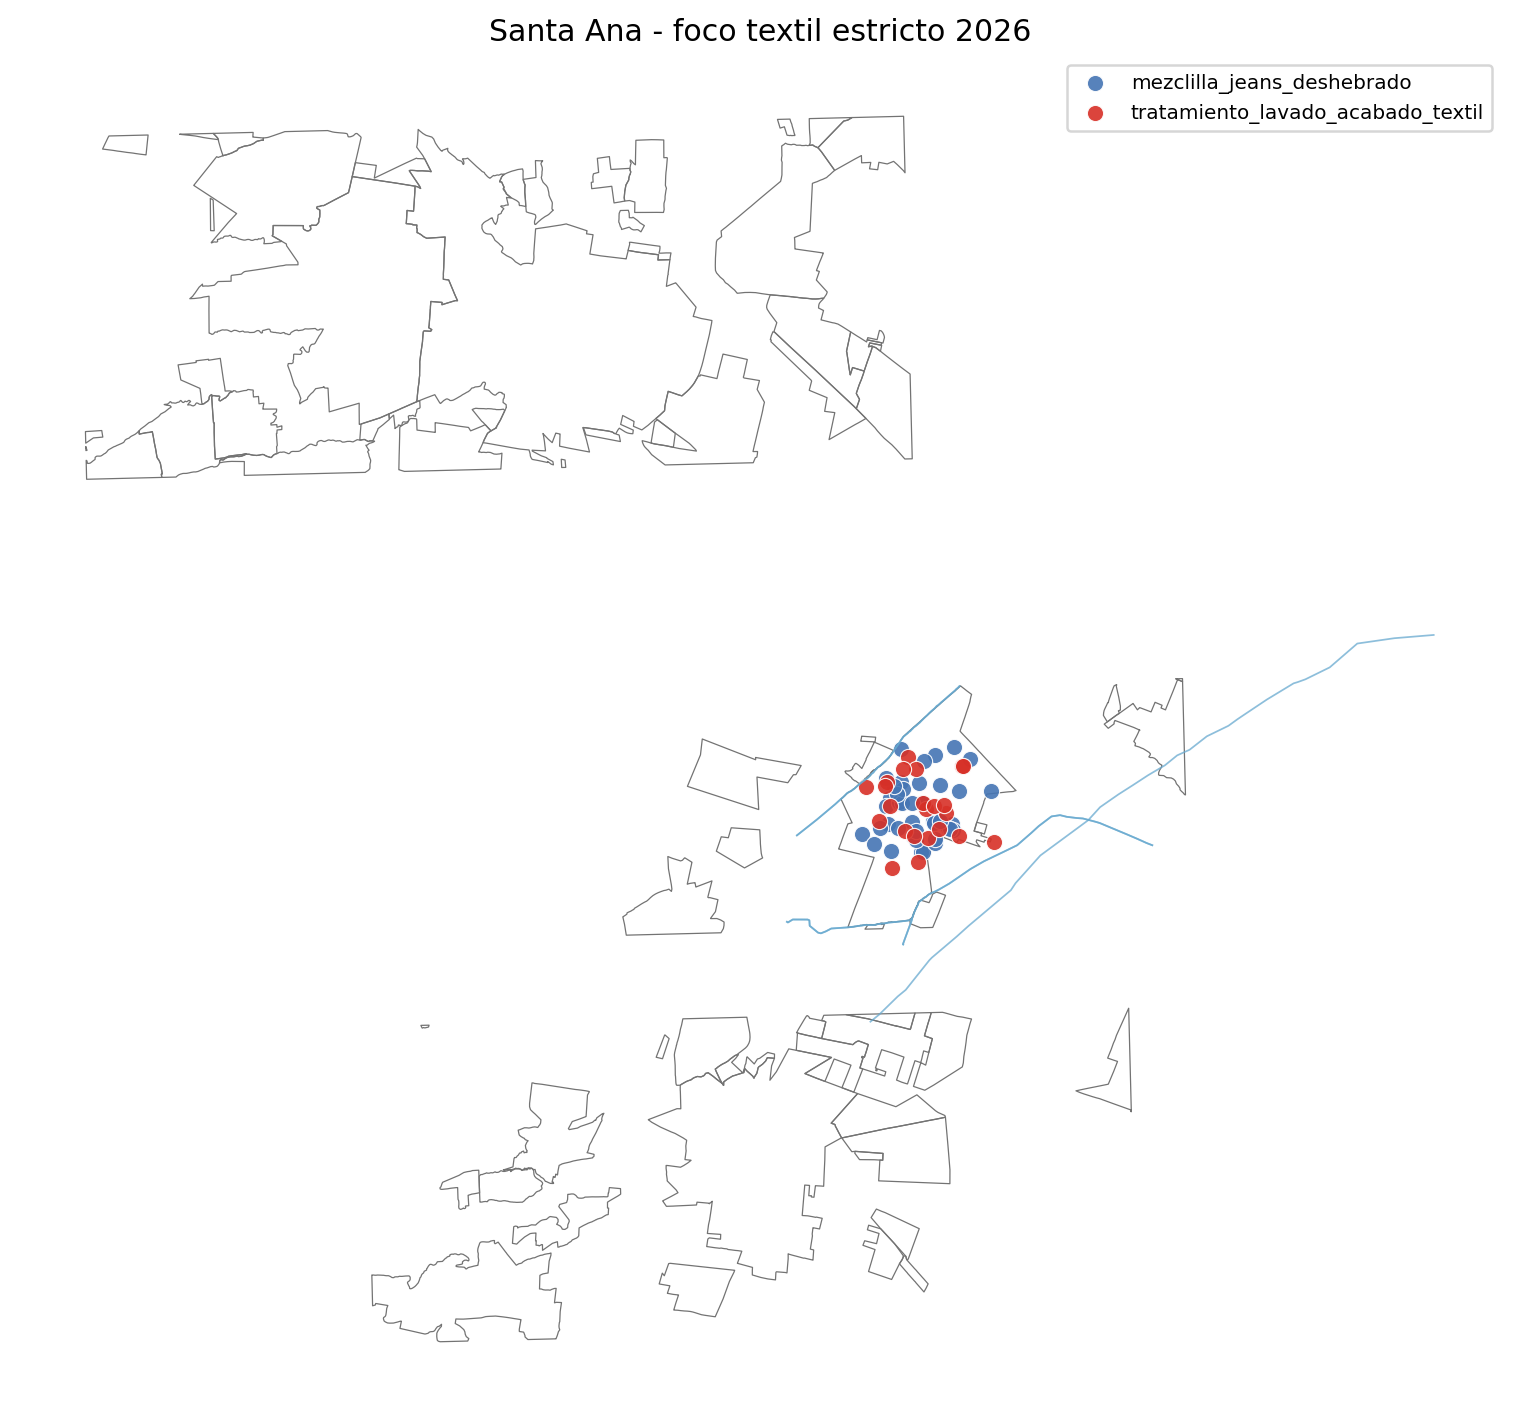
\includegraphics[width=0.95\linewidth]{../mapas/mapa_foco_textil_estricto_santa_ana.png}

\caption{Foco textil estricto Santa Ana 2026 por categoria.}

\end{figure}

\begin{figure}[h!]\centering

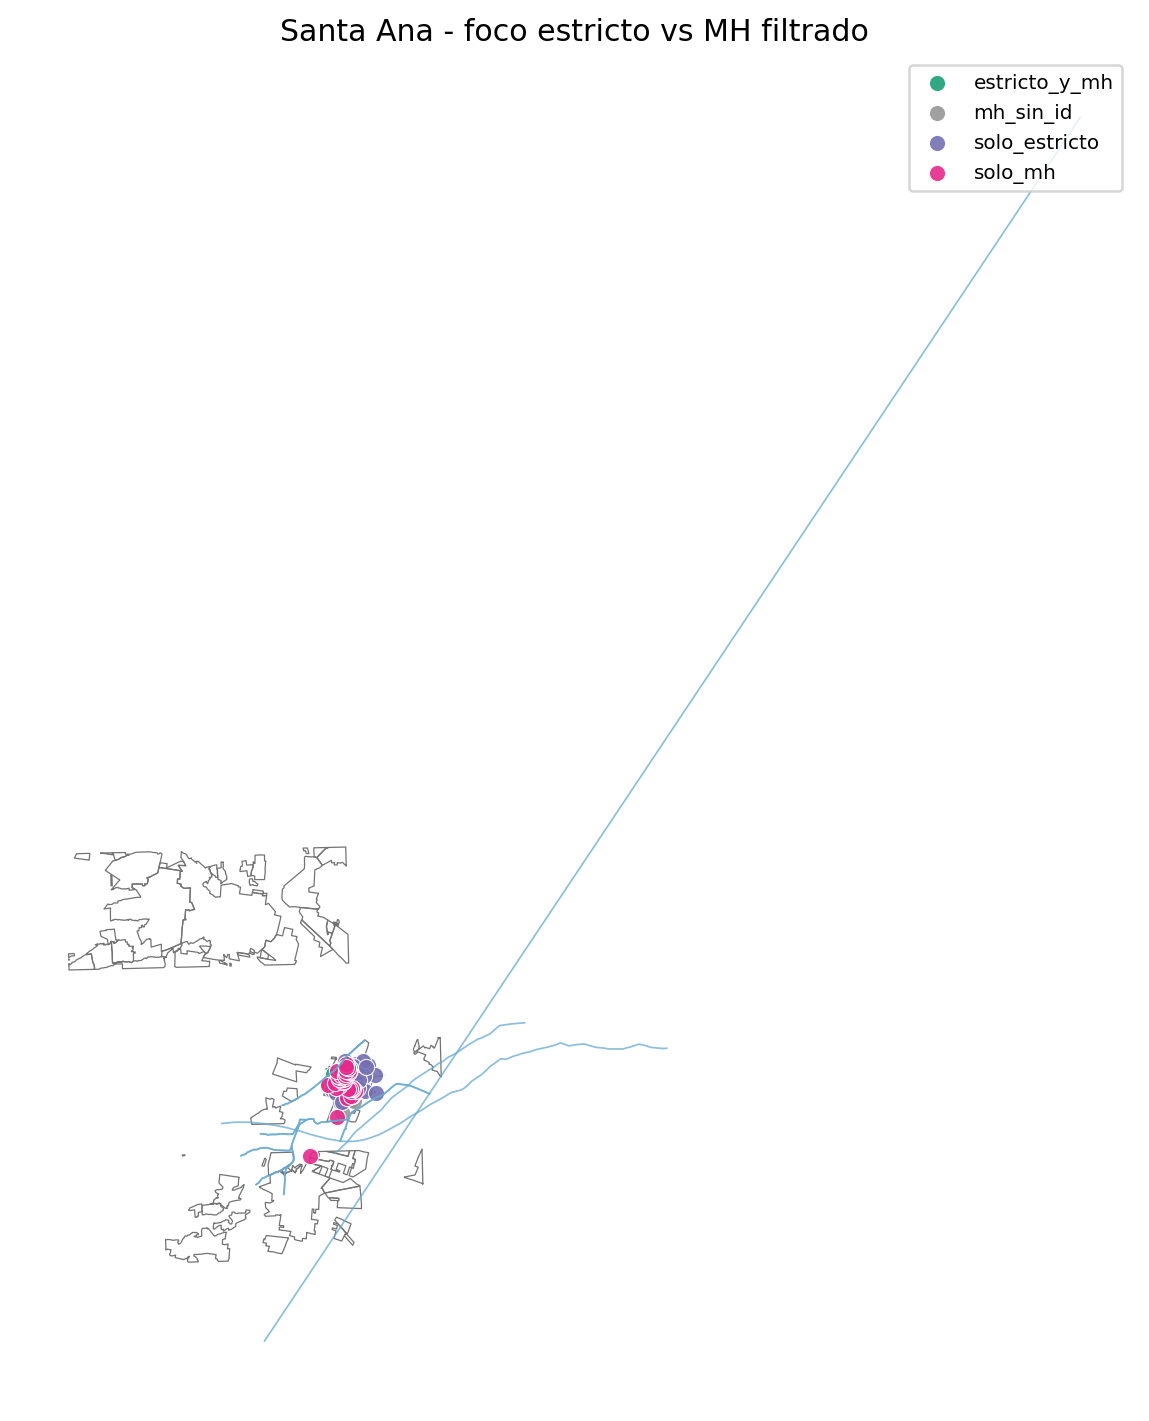
\includegraphics[width=0.95\linewidth]{../mapas/mapa_comparacion_estricto_vs_mh.png}

\caption{Comparacion entre foco estricto y capa MH filtrada.}

\end{figure}

\begin{figure}[h!]\centering

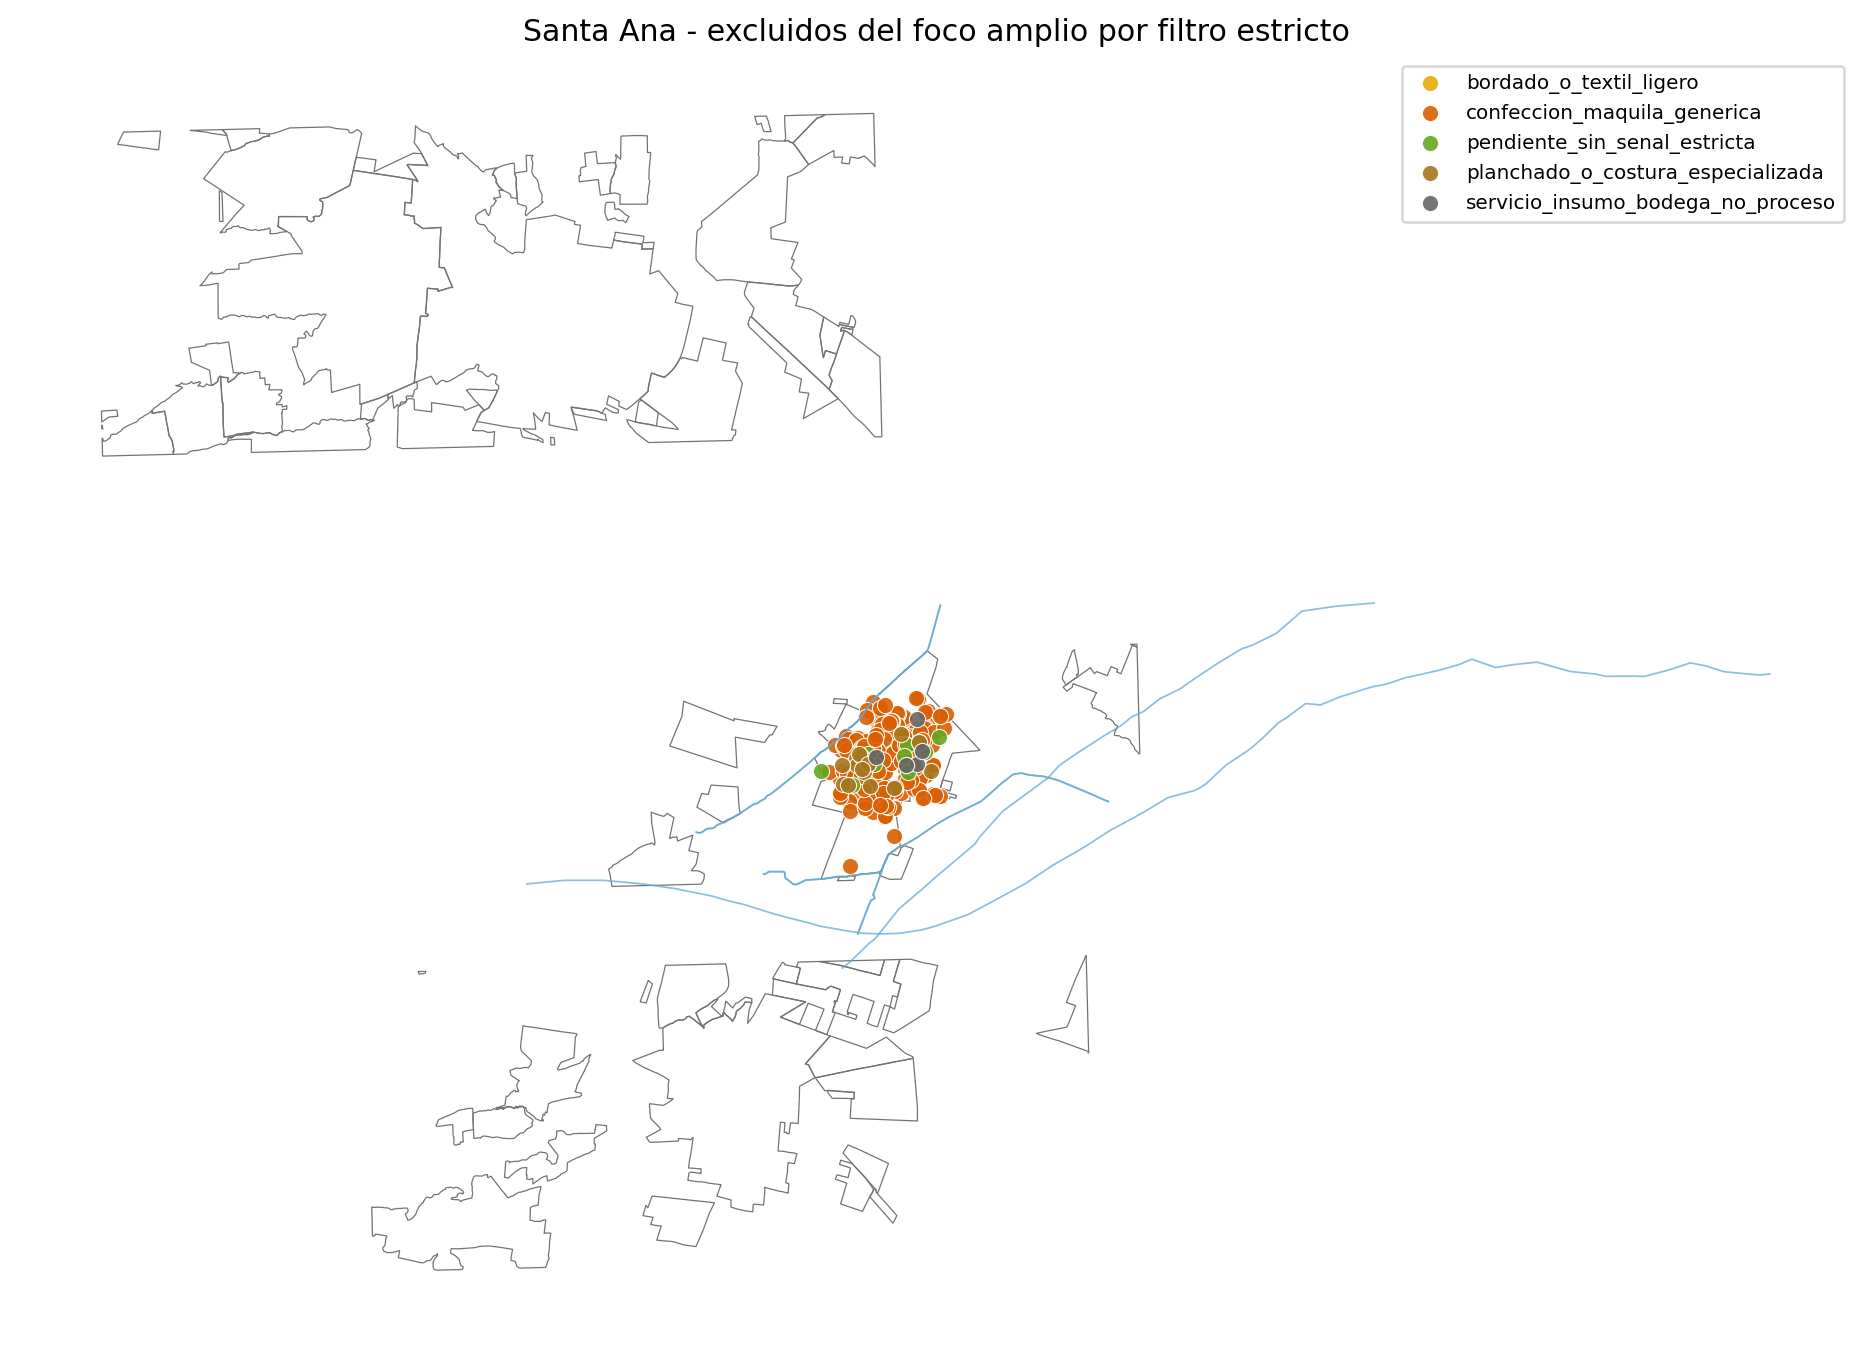
\includegraphics[width=0.95\linewidth]{../mapas/mapa_excluidos_del_foco_amplio.png}

\caption{Registros que salieron del foco amplio al aplicar el criterio estricto.}

\end{figure}

\section{Lectura}

La diferencia principal frente al foco amplio es que se retira la maquila/confeccion generica. Esto reduce ruido para una auditoria ambiental porque muchos talleres de ropa terminada no muestran, por si solos, senal de lavado, acabado, tratamiento, mezclilla o produccion material textil. La capa MH filtrada conserva una nocion mas amplia: solo una parte cruza con este foco estricto.

\section{Archivos generados}

\begin{itemize}

\item \texttt{capas\_qgis/foco\_textil\_estricto\_santa\_ana\_2026.gpkg}

\item \texttt{tablas/foco\_textil\_estricto\_santa\_ana\_2026.csv}

\item \texttt{tablas/excluidos\_del\_foco\_amplio\_santa\_ana.csv}

\item \texttt{mapas/mapa\_foco\_textil\_estricto\_santa\_ana.html}

\item \texttt{mapas/mapa\_comparacion\_estricto\_vs\_mh.html}

\item \texttt{mapas/mapa\_excluidos\_del\_foco\_amplio.html}

\end{itemize}

\end{document}